
\documentclass{article}
\usepackage[margin=1.0in]{geometry}
\usepackage{color}
\usepackage{caption}
\usepackage{hyperref}
\usepackage{csquotes}
\usepackage{amsmath}
\usepackage{amssymb}
\usepackage{soul}
\usepackage{changepage}
\usepackage{alg}
\usepackage{graphicx}
\graphicspath{ {./} }
\usepackage{listings}
\lstset{aboveskip=3mm, belowskip=3mm, showstringspaces=false, columns=flexible, basicstyle={\small\ttfamily}, numbers=none, breaklines=true, breakatwhitespace=true, tabsize=3}

\usepackage{newlfont}
\usepackage{program}
\catcode`\_\active

\newtheorem{randlang}{RandLang}[section]

\begin{document}
\begin{center}{\huge   Lab 1: Zipf's Law }\\[0.4cm]{\large  Philosophy of Computation }\\[0.75cm]{\large  Henry Blanchette }\\[0.5cm]{\large  February 8th, 2019 }\\[1.0cm]\end{center}\section{Real-World Corpus}

I used the provided \texttt{ doc2freq.py } and \texttt{ zipf.R } scripts to produce the Zipf plots for several real-world texts. I decided to use a variety in kinds of texts, to see if I could produce irregular Zipf correlations between word kinds and word tokens frequencies. I chose a couple novels, some computer code, an English dictionary (including definitions), the Bible, and a relatively small list of US city names. I hypothesized that the novels and the information-texts would segregate in their Zipf correlations. Figure 1 is the combined Zipf scatter-plot for all the mentioned texts. Also, just to be clear, \texttt{ 8cc } is a C-compiler, and \texttt{ patentsample } is the same patent text data given to us originally for this lab.


\begin{figure}[h]
\centering
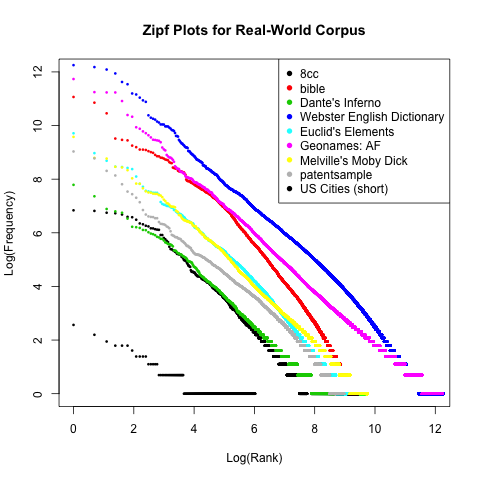
\includegraphics[width=13cm,keepaspectratio]{zipf-combined.png}
\captionsetup{labelformat=empty} \caption{Figure 1}
\end{figure}


I was surprised by how strongly Zip's law appears to hold for this diverse corpus. For all but the US Cities list, deviations from a $  -1  $ slope are very small and likely just noise from the small amount of data. I hypothesized that the US Cities list has a much shallower negative slope because it includes lots of unique words, as is expected for a list of names. And of course, the text has only 413 unique words.



However, another surprising result is that the Geonames list follows Zipf's law very well. The text is the set of names of cities in the world that start with AF, so most are not English or English-related. But even with such a mixture of languages, Zipf's law prevails.



From these results, I am moved to suspect that Zipf's law is a combinatorial result rather than a sociological or lingual one. I can't see any rhyme or reason connecting these texts together in Zipf's way. I explored this hypothesis to some degree in the next section.

\section{Random Languages}

In this section, I explore some random text generators and Zipf plots. The interesting question is of whether the same Zipf correlation that holds so consistently in real-world texts holds in random texts in the same way or at all. I took two main approaches to random text generations, which differed in how they sampled from the alphabet: uniformly or weighted by the actual distribution of English letters.

\subsection{Random Languages}

I use the term \textit{random language} to refer to an algorithm that, with certain parameters, produces random text that attempts to mimic certain features of real languages. I implemented a few different random languages in order to explore how different parameters affected the Zipf plots of the produced text.

\subsubsection{RandLang1}

The first random language chooses from the alphabet uniformly and from the whitespace character with a given probability. I implemented this via the following algorithm:
\vspace{0.4cm}
\subsubsection*{RandLang1}
\begin{adjustwidth}{1cm}{}\begin{programbox}
length := \mbox{the length (in characters) of text to generate}
\textit{space-chance} := \mbox{the chance for a generated character to be a space}
text := ``''
\FOR 1 \TO length \DO
  x := \mbox{a random number in } [0,1]
  \IF x < \textit{space-chance}
    \THEN c := \mbox{a random letter}
      text := text \concat x
    \ELSE text := text \concat `` ''
  \FI
\OD
\textbf{return } text
\end{programbox}\end{adjustwidth}
 \vspace{0.6cm}

For my experiments, a length of 1 million characters seemed to work well. I varied the \textit{space-chance} variable over the range $  0.1, 0.2, \dots, 0.9  $. The resulting Zipf plots for texts generated this way are combined in Figure 2.


\begin{figure}[h]
\centering
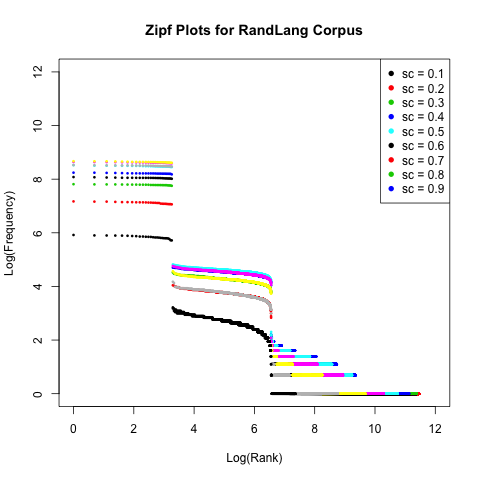
\includegraphics[width=13cm,keepaspectratio]{randlang-combined.png}
\captionsetup{labelformat=empty} \caption{Figure 2}
\end{figure}


The result here does not seem to achieve the expected $  -1  $ slope at all. There is a sort of rude trend in that direction, but the cubic-like curve in the center is not like anything seen in the real world corpus. Clearly, RandLang1's so simple of an approach will not be enough to create a realistic Zipf plot.

\subsubsection{RandLang2}

The second random language works similarly to the first, except that it chooses from the alphabet in a weighted fashion, using the same probability distributions for letters as the English languages. I used the distribution data provided by \href{https://www3.nd.edu/~busiforc/handouts/cryptography/letterfrequencies.html}{nd.edu/letterfrequencies}. I implemented this via the following algorithm:


\vspace{0.4cm}
\subsubsection*{RandLang2}
\begin{adjustwidth}{1cm}{}\begin{programbox}
P := \mbox{the actual distribution of English letters}
length := \mbox{the length (in characters) of text to generate}
\textit{space-chance} := \mbox{the chance for a generated character to be a space}
text := ``''
\FOR 1 \TO length \DO
  x := \mbox{a random number in } [0,1]
  \IF x < \textit{space-chance}
    \THEN c := \mbox{a random letter, weighted by } P
      text := text \concat c
    \ELSE text := text \concat `` ''
  \FI
\OD
\textbf{return } text
\end{programbox}\end{adjustwidth}
 \vspace{0.6cm}

Producing 1 million characters in RandLang2 takes much longer than in RandLang1 because choosing from a weighted distribution is more computationally-costly, so I used a length of just 100,000 for my experiments here. Again, I varied the \textit{space-chance} variable over the range $  0.1, 0.2, \dots, 0.9  $. The resulting Zipf plots for texts generated this way are combined in Figure 3.


\begin{figure}[h]
\centering
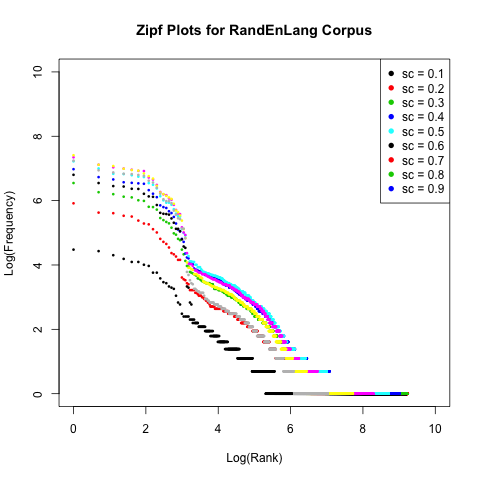
\includegraphics[width=13cm,keepaspectratio]{randenlang-combined.png}
\captionsetup{labelformat=empty} \caption{Figure 3}
\end{figure}


This looks much better than RandLang1 after just one change. This made me hopeful that there is, in fact, much I could do to improve my random mimics of realistic Zipf plots with just a few changes. I decided to make just one more change in the scope of this lab.

\subsubsection{RandLang3}

The third random language uses the same strategy as RandLang2 for choosing characters, but instead of using chance to choose a whitespace, RandLang3 randomly decides the length of each word individually. The lengths are chosen from the word-length distribution of the Bible text. (which I used in the Real-World Corpus section). It is depicted in Figure 4.


\begin{figure}[h]
\centering
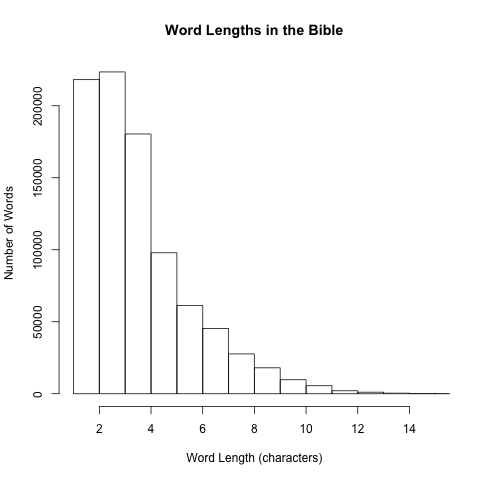
\includegraphics[width=13cm,keepaspectratio]{word-lengths-bible.png}
\captionsetup{labelformat=empty} \caption{Figure 4}
\end{figure}


My hypothesized that a large problem with the strategies of the previous two languages had to do with the fact that their generated text massively over-represents large words (e.g. larger than 8 letters or so) as compared to real-world texts' representation of large words. So, perhaps taking into account the actual distribution of words could make a relevant difference. The algorithm for RandLang3 is implemented by the following algorithm:


\vspace{0.4cm}
\subsubsection*{RandLang3}
\begin{adjustwidth}{1cm}{}\begin{programbox}
P := \mbox{the actual distribution of English letters}
L := \mbox{the distribution of word lengths in the Bible}
length := \mbox{the length (in words) of text to generate}
text := ``''
\FOR 1 \TO length \DO
  \textit{word-length} := \mbox{a random length, weighted by } L
  \FOR 1 \TO \textit{word-length} \DO
    c := \mbox{a random letter, weighted by } P
    text := text \concat c
  \OD
\OD
\textbf{return } text
\end{programbox}\end{adjustwidth}
 \vspace{0.6cm}

I found that generating about 100,000 words from RandLang3 took a reasonable amount of time. Additionally, I didn't need to vary a \textit{space-chance} variable this time, so there is only one trend to consider. The resulting Zipf plot for text generated by RandLang3, alongside a few real-world texts for reference, are combined in Figure 5.


\begin{figure}[h]
\centering
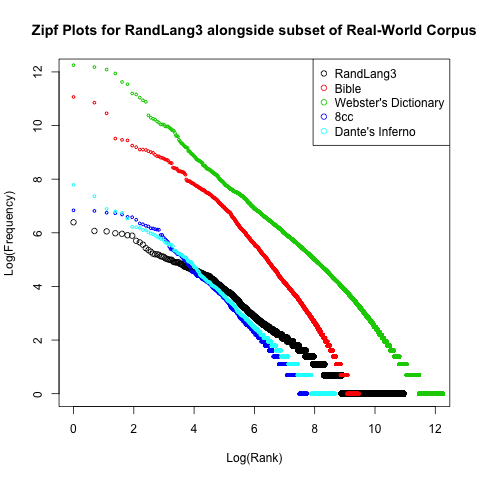
\includegraphics[width=13cm,keepaspectratio]{randlengths-real.png}
\captionsetup{labelformat=empty} \caption{Figure 5}
\end{figure}


This result was particularly exciting. It seemed that the adjustment for word-length distribution did a lot in the way of making RandLang3 realistic in its Zipf plot. It does, however, seem to have a much shallower slope than $  -1  $, perhaps something more like $  -0.75  $. But in overall shape it is a huge improvement over the previous RandLang1, and RandLang2. RandLang3's Zipf plot even in virtually indistinguishable from some real-world texts like \textit{Dante's Inferno} and \textit{8cc}.

\section{Conclusions}

The shape of RandLang1's and RandLang2's Zipf plots are very different from the real-world corpus's, but the transition in shape from RandLang1 to RandLang2 is one towards more realism rather than away from, and this suggests that there could be a few other commons features of language that could be added to my algorithms to make the shape even more like the real-world Zipf plots.



The variance in \textit{space-chance} directly influences average word size, and in the Zipf plot this is reflected by the distance from the origin. The larger the words, the further from the origin the Zipf plot. This brings a new analytical perspective to the real-world plots where there was also some clear stratification in distance from the origin. For example, Webster's English Dictionary was the furthest from the origin while 8cc was closest (excluding the outlier). I think this makes sense because the dictionary contains lots of large words by default, as they must be included if they are English, whereas in programming languages, especially systems-level programming such as a compiler, there are lots of short words and numbers that are often separated by grammatical characters that are excluded after cleaning.



However, this hypothesis on word lengths is not well-supported by the results from RandLang3. RandLang3 uses the same distribution of word lengths as the Bible, yet has a plot much closer to the origin than the Bible's plot. Though the plots to converge towards their higher ranking words' frequencies.



RandLang3 has around a $  -0.75  $ slope, which is significantly far from the Zipf-expectation of $  -1  $, but is still very close to some other real-word texts that I included in the first section (see Figure 5 for a side-by-side comparison). What is there to make of this? Clearly, the distribution of letters and word lengths in the text is highly important to the Zipf-shape, so Zipf relationship between word frequency and rank is not merely a combinatorial observation of noise. My experiments did not delve into possible reasons or reverse-engineering strategies for producing these needed a-priori distributions, but I'm sure there is more there to look into.



My main result is that I can produce relatively-realistic Zipf plots randomly if given realistic word-length and letter distributions, but that the generated text will have a slightly shallower slope than predicted by Zipf. Given my success in developing the final algorithm, RandLang3, from the very unrealistic RandLang1 just by accounting for realistic word-length and character distributions suggests that those and perhaps just a few other features are mainly responsible for the Zipf phenomenon.





\end{document}